\chapter{Evaluación del Impacto Ambiental}
\begin{definition}[Impacto ambiental]
    Es un instrumento de la Política Ambiental, cuyo objetivo es prevenir, modificar y restaurar los daños al ambiente así como la regulación de obras o actividades para evitar o reducir sus efectos negativos en el ambiente (figura \ref{ia1}).
\end{definition}
\begin{figure}[h!]
\centering
    \smartdiagramset{priority arrow width=2cm,
    priority arrow height advance=2.25cm,
    priority arrow head extend=0.3cm}
    \smartdiagram[priority descriptive diagram]{Políticas,Planes y Programas,Proyectos}
  \caption{La evaluación ambiental es un enfoque preventivo de gestión ambiental orientado a conseguir el desarrollo sostenible}
  \label{ia111}
\end{figure}
\begin{enumerate}
    \item Por utilización de recursos naturales \begin{enumerate}
        \item Renovables
        \item No renovables
    \end{enumerate}
    \item Por ocupación del territorio \begin{enumerate}
        \item Suelo y agua
    \end{enumerate}
    \item Por contaminación \begin{enumerate}
        \item Aire
        \item Agua y
        \item Suelo.
    \end{enumerate}
\end{enumerate}
\begin{figure}[h!]
% \centering
    \smartdiagramset{border color=none,
    set color list={blue!50!cyan,green!60!lime,orange!50!red,red!80!black},
    back arrow disabled=true}
    \smartdiagram[flow diagram:horizontal]{LIMITES, Tasa de\\ renovación, Tasa de consumo o de sustitución, Capacidad de carga, Cap. de dispersión, Cap. de dilución, Cap. de recepción}

    \smartdiagramset{border color=none,
    set color list={blue!50!cyan,green!60!lime,orange!50!red,red!80!black},
    back arrow disabled=true}
    \smartdiagram[flow diagram:horizontal]{OBJETIVOS, Evitar la sobreecplotación, Evitar el agotamiento, Evitar la sobrecarga, Evitar contaminación arriba del límite}

    \smartdiagramset{border color=none,
    set color list={blue!50!cyan,green!60!lime,orange!50!red,red!80!black},
    back arrow disabled=true}
    \smartdiagram[flow diagram:horizontal]{META, desarrollo sustentable}
  \caption{Criterios de sustentabilidad por tipo de impacto ambiental.}
  \label{i2}
\end{figure}
Los impactos ambientales de los proyectos hidráulicos que podemos destacar son principalmente:
\begin{itemize}
    \item Interrumpen la conectividad de los sistemas fluviales. Esto interfiere en la reproducción y la migración de los peces y fauna acuática
    \item Modifican el transporte de sediments que impacta principalmente los deltas
    \item Alteran el régimen de flujo natural.
\end{itemize}
Marco de referencia: La conferencia de Estocolmo de 1972 centraba la atención internacional en temas medio ambientales, especialmente los relacionados con la degradación ambiental y la contaminación transfronteriza

Publicación y entrada en vigor de la LGEEP en 1988, estableció un parte aguas en la gestión ambiental de México
\begin{figure}[h!]
\centering
  \includegraphics[width=0.5\textwidth]{ia1.jpg}    
  \caption{Evolución de la legislación e institucionalidad ambiental en México}
  \label{ia1}
\end{figure}
\begin{figure}[h!]
\centering
  \includegraphics[width=0.5\textwidth]{ia3.png}
  \caption{Evaluación de la LGEEP y leyes correlacionadas}
  \label{ie3}
\end{figure}
% Peso específico del concreto es de $2400kg/m^2$
\subsection{Cumbres y acuerdos mundiales}
las cumbres sirven para llegar a acuerdos, firmar compromisos y luchar conjuntamente en pro del ambiente.

Estocolmo, Suecia en 1972 realizó el primer foro mundial sobre medio ambiente, siendo un programa de las Naciones Unidas. Fue una declaración intergubernamental de principios y propuestas para una sociedad sostenible, solidaria y justa en materia de educación ambiental, visibilizando los problemas ambientales y sus consecuencias.
\begin{itemize}
    \item Convenio de Viena
    \item Protocolo de Monreal
    \item Cumbre de la tierra Río 1992 \begin{itemize}
        \item Comunidad científica, Sociedad civil y líderes políticos
        \item 125 jefes de Estado y de Gobierno
        \item Presentó el desarrollo sustentable como eje de desarrollo
        \item La protección del medio ambiente debe ser parte del proceso de desarrollo
    \end{itemize}
    \item Protocolo de Kioto \begin{itemize}
        \item Estrecha relación con el Protocolo de Montreal
        \item Evitar emitir $CO_2$
        \item Define el problema de cambio climático
        \item Instrumento legal para combatirlo
    \end{itemize}
    \item Cumbre mundial sobre desarrollo sustentable (Johannesburgo, Sudáfrica 2002) \begin{itemize}
        \item Verifica los avances de la Cumbre de Rio 1992
        \item Invita a la iniciativa privada a unirse a los acuerdos
        \item Invita a fortalecer lazos entre gobierno
    \end{itemize}
    \item Cumbre de Copenhague (Dinamarca, 2009) \begin{itemize}
        \item Confrontación entre países desarrollado en contra de los países en vías de desarrollo
        \item No estableció una agenda vinculante
    \end{itemize}
    \item Conferencia sobre el cambio climático (Cancún, México 2010) \begin{itemize}
        \item Acuerdo jurídicamente vinculante sobre clima con aplicación 2012 (Copenhague 2009) fracasó en encontrar un acuerdo
        \item Creación de un Fondo verde para financiar proyectos en beneficio del ambiente.
    \end{itemize}
    \item Río de Janeiro, 2012 \begin{itemize}
        \item Evaluar avances de Río 1992
        \item Asegurar un renovado compromiso político para el desarrollo sustentable
        \item Se centra en economía verde y el marco de referencia institucional para un desarrollo sostenible.
    \end{itemize}
    \item Objetivos de desarrollo sostenible (Nueva York, 2015) \begin{itemize}
        \item Fin de la pobreza
        \item Hambre cero
        \item Salud y bienestar
        \item Especialidad de calidad
        \item Igualdad de género
        \item Agua limpia y saneamiento
        \item Energía asequible y no contaminante
        \item Trabajo decente y crecimiento económico
        \item Industria, innovación e infraestructura
        \item Reducción de las desigualdades
        \item Ciudades y comunidades sostenibles
        \item Producción y consumo responsables
        \item Acción por el clima
        \item Vida submarina
        \item Vida de ecosistemas terrestres
        \item Paz, justicia e instituciones sólidas
        \item Alianzas para lograr los objetivos.
    \end{itemize}
    \item Conferencia de las Naciones Unidas sobre Cambio Climático (Francia, París 2015) \begin{itemize}
        \item Logró definir nuevo pacto que sustituye al de Kioto 1997
        \item Consolidar la Economía Verde
    \end{itemize}
\end{itemize}
De las obras o actividades que requieren autorización en materia de impacto ambiental y de las excepciones
\begin{enumerate}
    \item Exploración, explotación y beneficio de minerales y sustancias reservadas a la federación
    \item Instalaciones de tratamiento, confinamiento o eliminación
\end{enumerate}
Del artículo 5to - hidráulicas:

Quienes pretendan llevar a cabo alguna
\begin{itemize}
    \item Depósito o relleno con materiales para ganar terreno al mar
    \item Drenaje y desecación de cuerpos de aguas
    \item Modificación o entubamiento de cauces
    \item Obras de dragado de cuerpos de agua
    \item Plantas potabilizadoras
    \item Plantas desaladoras
\end{itemize}


\begin{definition}[Definición de la Evaluación de Impacto Ambiental]
    Es un instrumento de la política ambiental, cuyo objetivo es prevenir, mitigar y restaurar los daños ambientales así como la regulación de obras o actividades para evitar o reducir sus efectos negativos en el medio ambiente.
\end{definition}
Contenido de una Manifestación de Impacto Ambiental

El objetivo de la evaluación del impacto ambiental es la sustentabilidad, pero para que un proyecto sea sustentable debe considerar además la factibilidad económica y el beneficio social, el aprovechamiento razonable de los recursos naturales.

El procedimiento de evaluación de impacto ambiental: 

Lo realiza la autoridad mediante un procedimiento de tipo técnico administrativo, hay tres opciones mediante las cuales puede presentarse dependiendo del control que se tenga sobre los impactos y la magnitud del área donde se pretende desarrollar un proyecto:
\begin{itemize}
    \item Informe preventivo
    \item Manifestación de impacto ambiental modalidad particular y 
    \item Manifestación de impacto ambiental modalidad regional
\end{itemize}


\subsubsection{Informe preventivo}
Requieren de presentar un informe preventivo y no manifestación de impacto ambiental en los siguiente casos:
\begin{itemize}
    \item Existan normas oficiales Mexicanas u otras disposiciones que regulen las emisiones, las descargas, el aprovechamiento de recursos naturales y, en general, todos los impactos ambientales relevantes que puedan producir las obras o actividades
    \item Las obras o actividades de que se trate estén expresamente previstas por un plan parcial de desarrollo urbano o de ordenamiento ecológico que hay sido evaluado por la Secretaría en los términos del artículo siguiente o
    \item Se trate de instalaciones ubicadas en parques industriales autorizados en los términos de la presente sección
\end{itemize}
En los casos anteriores, la Secretaría una vez analizando el informe preventivo, determinará, en un plazo no mayor a 20 días si se requiere la presentación de una manifestación de impacto ambiental en alguna de las modalidades o si se está en alguno de los supuestos señalados

\subsubsection{Manifestación de impacto ambiental} 

Se trata de un documento con base en estudios técnicos on el que las personas (físicas o morales) que desean realizar alguna de las obras o actividades previstas en el artículo 28 de la LGEEPA, analizan y describen las condiciones ambientales anteriores a la realización del proyecto con la finalidad de evaluar los impactos potenciales que la construcción y operación de dichas obras o la realización de las actividades podría causar al ambiente y definir y proponer las medidas necesarias para prevenir, mitigar o compensar esas alteraciones.

El contenido de una manifestación de impacto ambiental depende de la modalidad que requiere, en la siguiente figura:
% TODO:
% \begin{table}[h!]
%     \centering
%     \begin{tabular}{@{}ccc@{}}
%     \toprule
%     \begin{tabular}[c]{@{}c@{}}Orden\\ de\\ gobierno\end{tabular} &
%       \begin{tabular}[c]{@{}c@{}}Tipos\\ de MIA\end{tabular} &
%       Actividades que requieren \\ \midrule
%     \multirow{2}{*}{Federal} &
%       Regional &
%       \begin{tabular}[c]{@{}c@{}}\begin{itemize} \item Parques industriales \item Parques acuícolas \item Granjas acuícolas de más de 500 hectáreas     \item Carreteras     \item Vías férreas \item Proyectos de generación de energía nuclear     \item Presas     \item Proyectos que alteran las cuencas hidrológicas \item Planes o programas parciales de desarrollo urbano o de ordenamiento ecológico     \item Conjunto de proyectos de obras y actividades que pretendan realizarse en una región ecológica determinada \item Proyectos que pretendan desarrollarse en sitios en que se pudieran ocasionar la destrucción, el aislamiento o la fragmentación de los ecosistemas. \end{itemize}\end{tabular} \\
%      &
%       Particular &
%       \begin{tabular}[c]{@{}c@{}}\begin{itemize}\item Demás casos, previstos en el artículo 5 del reglamento de la LGEEPA en materia de EIA \end{itemize}\end{tabular} \\
%     Estatal &
%       \multicolumn{2}{c}{\multirow{2}{*}{\begin{tabular}[c]{@{}c@{}}\begin{itemize} \item Depende de cada legislación estatal municipal \end{itemize}\end{tabular}}} \\
%     Municipal &
%       \multicolumn{2}{c}{} \\ \bottomrule
%     \end{tabular}
%     \caption{Tipos de M.I.A.}
%     \label{tabei}
% \end{table}
\subsection{Manifestación del Impacto Ambiental}
La evaluación del impacto ambiental es el procedente

% Alcances del PEIA:
% \begin{itemize}
%     \item Cumplimiento normativo y vinculación con otros instrumentos
%     \item Considerar as
% \end{itemize}
\begin{definition}[MIA]
    Documento mediante el cual se da a conocer, con base en estudios el impacto ambiental, significativo y potencial que generaría una obra o actividad, así como la forma de evitarlo o atenuarlo en caso de que sea negativo
\end{definition}
\subsubsection{Proceso administrativo normativo}
\begin{enumerate}
    \item Genera proyecto de inversión
    \item Revisar la LGEEPA y el reglamento para determinar si debe ingresar PEIA
    \item Elaborar MIA
    \item Promovente ingresa MIA a EIA
    \item Revisión preliminar de acuerdo con el marco legal
    \item Se publica en gaceta y se abre a la consulta publica
    \item Inicia revisión en áreas especializadas
    \item Solicitud de información adicional evaluación de impactos y de medidas de mitigación; consulta institucionales y municipios
    \item Emisión de resolutivo: solicitud de garantías
    \item Inspección y vigencia PROFEPA PEIA (artículo 55)
    \item Inicia proyecto según disposiciones del plan de manejo ambiental, seguimiento de condicionales
\end{enumerate}
\subsubsection{Actores en el procedimiento de EIA}
\begin{itemize}
    \item Promovente consultor \begin{itemize}
        \item Interesados, en la elaboración de planeación IP o MIA \begin{itemize}
            \item Definición del proyecto e identificación de alternativas
            \item Pre-evaluación
            \item Identificación de requerimientos y alcances
            \item Descripción de área de influencias
            \item Análisis de impactos ambientales
            \item Identificación, valorización y jerarquización
            \item Plan de manejo ambiental: Programa de mitigación reparación, compensación de prevención de riesgos y contingencias
            \item Documento formal (IP o MIA)
        \end{itemize}
    \end{itemize}
    \item Autoridad \begin{itemize}
        \item Afectados, en el control y seguimiento; dictaminación: \begin{itemize}
            \item Revisión de documento formal y soporte legal
            \item Consulta y participación ciudadana
            \item Toma de decisión y resolución
            \item Establecimiento de plan de manejo ambiental
            \item Verificación del plan de manejo ambiental y retroalimentación.
        \end{itemize}
    \end{itemize}
\end{itemize}
\begin{figure}[h!]
\centering
  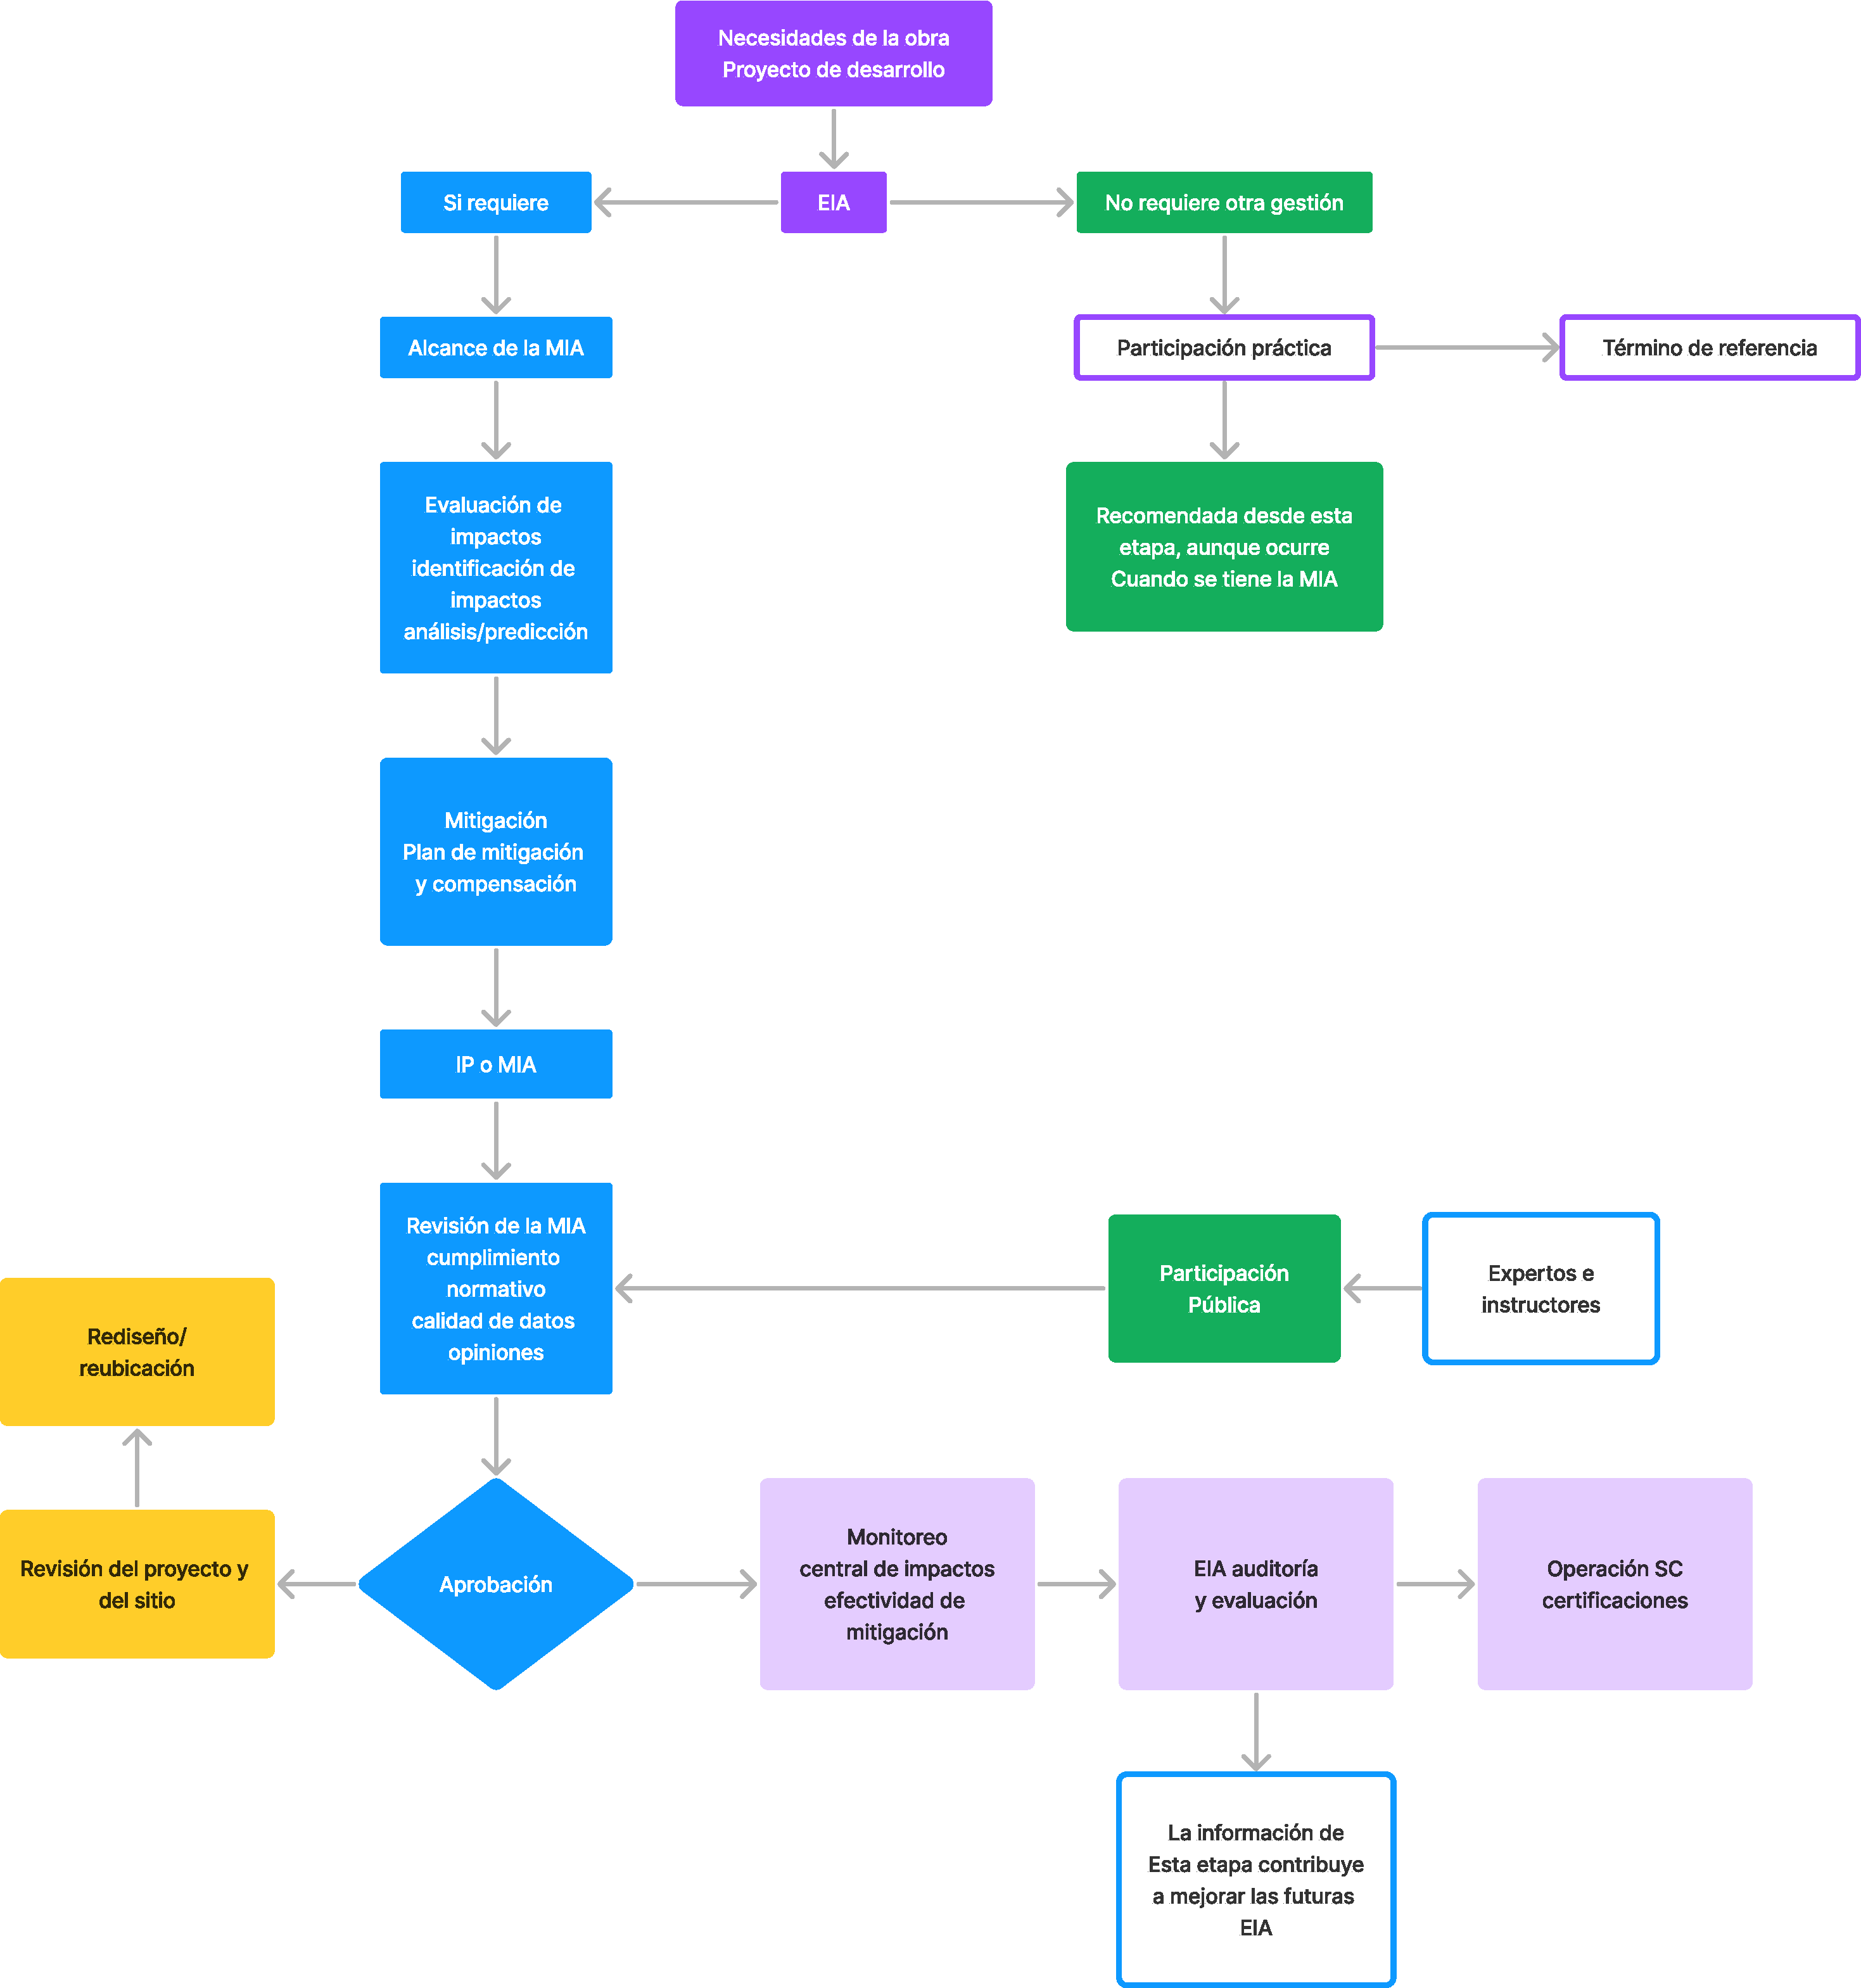
\includegraphics[width=0.8\textwidth]{ia2.pdf}
  \caption{Necesidad de la obra}
  \label{ia2}
\end{figure}
\subsubsection{Elementos ambientales, Tipología y terminología}
Los elementos están conformados por:
\begin{itemize}
    \item Adyacentes
    \item del Proceso
    \item Intrínsecos
\end{itemize}

\subsubsection{Elementos adyacentes}
Son los elementos necesarios a considerar,
\begin{itemize}
    \item Medio ambiente
    \item Medio físico o medio natural \begin{itemize}
        \item Medio inerte: Agua, suelo y aire
        \item Medio biótico: Flora y Fauna
        \item Medio perceptual: unidades de paisaje
    \end{itemize}
    \item Medio socioeconómico
    \item Factores ambientales \begin{itemize}
        \item Hombre, flora y Fauna
        \item Suelo, aire, clima, paisaje, interacciones
        \item Bienes materiales y el patrimonio cultural
    \end{itemize}
    \item Ecología
    \item Proyecto
    \item Titular del proyecto
    \item Entorno de un proyecto
    \item Capacidad de acogida
    \item Gestión ambiental
    \item Autoridad competente
    \item Autoridad competente medio ambiente
\end{itemize}
Por la variación de la CA, un impacto positivo potencia las condiciones naturales ecológico geográficas, cuando uno negativo en detrimento de valor naturalístico, estético, paisajístico, aumento de los perjuicios derivados de la contaminación.

Intensidad o grado de destrucción: impacto notable o muy alto; impacto mínimo y el impacto medio

Si es por la extensión, entonces Impacto puntual (muy localizado); impacto parcial (incidencia apreciable), impacto extremo, impacto determinante

Por el momento en que se manifiesta: Impacto latente (Aportación progresiva de sustancias), impacto inmediato (Efecto a tiempo=0) y el impacto a momento crítico (independiente del plazo de manifestación)

Por su persistencia: Impacto temporal y permanente.

Por la relación causa y efecto: Impacto indirecto o secundario.

Por su capacidad de recuperación: Impacto irreversible, reversible, mitigable y fugaz.

Por la interrelación de acciones y efectos: Impactos simple, acumulativo y sinérgico

Por su periodicidad: Impacto continuo, discontinuo, periódico, y de aparición irregular.

Por las necesidades de aplicación de medidas correctivas: Impacto ambiental crítico, severo y moderado.

\subsubsection{Tipología de las Evaluaciones de Impacto Ambiental}
Los grupos se encuentran como:
\begin{itemize}
    \item Factores físico químicos
    \item Biológicos
    \item Paisajísticos
    \item Uso de suelo
    \item Estructura, infraestructura
    \item Sociales, culturales y humanos
    \item Económicos
\end{itemize}
Los factores medio ambientales son: Clima, agua, suelo, flora, fauna, valores culturales, etc.

Metodologías:
\begin{itemize}
    \item Diversidad en los factores afectados
    \item Existen diversas metodologías para evaluar un solo factor
    \item Un método según la actividad.
\end{itemize}

La matriz de Leopold: 100 acciones y 88 factores ambientales
\subsubsection{Valor ecológico}
Estará dado por las características propias del subsistema o en función de sus elementos constituyentes o factores del medio y de los procesos que los relacionan. Los factores o elementos constituyentes pueden ser inertes (factores del medio) y o los seres vivos (medios bióticos)

El valor de los factores inertes estriba, principalmente en su importancia en interés para la ciencia, la técnica, la cultura, la satisfacción humana y la calidad de vida:
\begin{itemize}
    \item La cantidad de la atmósfera, la ausencia de ruidos, la pureza del agua, el valor geomorfológico, yacimientos paleontológicos, dotan a un lugar de un valor que se deba preservar
    \item El valor de los factores del medio biótico (flora y fauna), se basa cualitativa y cuantitativamente en la reserva genética depositada en ellos
    \item Polinización, control natural de plagas, traslado de energía a través de las cadenas tróficas, alteración de hábitats y pérdida de especies.
\end{itemize}
\subsubsection{Valor productivo}
El medio ambiente en general y cada sistema o ecosistema en particular, producen bienes o servicios, en mayor o menor medida, dependiendo de la productividad y el equilibrio del mismo (desarrollo sostenible)

La producción es en forma de bienes tangibles (materias primas, agua, oxígeno, biomasa, alimentos, fármacos) e intangibles (depuración natural y reciclado de agua, recarga de acuíferos y regulación atmosférica, sosiego y tranquilidad de un paraje, canto de las aves).

\subsubsection{Valor paisajístico}
Se refiere a sus valores perceptuales, incluyendo consideraciones de orden estético, plásticos y emocionales del medio natural.

El valor paisajístico tendrá en cuenta:
\begin{itemize}
    \item La visibilidad o territorio que puede apreciarse desde una zona o punto determinado (cuenca visual)
    \item La calidad paisajística
\end{itemize}
\begin{definition}[Signo]
    Hace alusión al carácter beneficioso o perjudicial de las distintas acciones que van a actuar sobre los distintos factores considerados. El impacto se considera positivo cuando el resultado de la acción sobre el factor ambiental considerado produce una mejora de la calidad ambiental de este último. Por ejemplo el control de la erosión gracias a la plantación forestal con especies dedicadas en una zona federal.
\end{definition}

\begin{definition}[Intesidad]
Este término se refiere al grado de incidencia de la acción sobre el factor, en el ámbito específico en el que actúa. El baremo de valoración estará comprendido entre 1 y 12, en el que 12 expresará una destrucción total del factor en el área en la que se produce el efecto y el 1 una afección mínima.
\end{definition}
Es importante matizar que no se debe vincular, ni confundir, la intensidad de un impacto a la extensión de este. La intensidad se refiere al grado de destrucción del factor ambiental y la extensión a la cantidad de factor sobre la que se produce el efecto
\begin{itemize}
    \item Impacto de Baja o Mínima intensidad: 1
    \item Impacto de Moderada Intensidad: 4
    \item Impacto de Alta intensidad: 8
    \item Impacto de Muy Alta Intensidad: 12
\end{itemize}
\begin{definition}[Extensión (EX)]
Se refiere al área de influencia teórica del impacto en relación con el entorno del Proyecto dividido el porcentaje del área, respecto al entorno, en que se manifiesta el efecto.
\end{definition}
% Si la acción produce un efecto muy 
% \begin{itemize}
%     \item 
% \end{itemize}
Puntual: Solo se presenta en el lugar en donde aparece la acción del proyecto

Parcial/Local: Abarca el sitio del proyecto y zonas aledañas

Extenso/Regional: Trasciende a la localidad y se proyecta en una región más amplia
\begin{definition}[Momento (MO)]
El plazo de manifestación del impacto alude al tiempo que trascurre entre la aparición de
la acción ($t_0$) y el comienzo del efecto ($t_j$) sobre el factor del medio considerado.
\end{definition}
Este criterio califica el momento de ocurrencia del impacto con respecto a la acción que lo genera
\begin{itemize}
    \item Impacto a largo plazo(1)> 10 años
    \item Impacto mediano plazo (2) 1-10 años
    \item Impacto a Corto Plazo (3) <1 año
    \item Impacto inmediato (4) menor tiempo
\end{itemize}
% En este criterio se asume que los impactos inmediatos son de mayor relevancia pues requieren, paralela 
\begin{definition}[Persistencia (PE)]
    Se refiere al tiempo que permanecería el efecto desde su aparición y a partir del cual el factor afectado retornaría a las condiciones iniciales previas a la acción por medios naturales o mediante la introducción de medidas correctoras.
\end{definition}
\begin{itemize}
    \item Impacto fugaz o momentáneo 1(<1 año)
    \item Impacto temporal 2(1-10 años)
    \item Impacto Persistente 3(11-15 años)
    \item Impacto Permanente 4(>15 años)
\end{itemize}

El impacto temporal permanece sólo por un tiempo limitado, haya finalizado o no  la acción. Por ejemplo, la contaminación en Sonora tiene vigencia sólo durante la emisión del sonido (acción finalizada). la contaminación de Río, en una zona determinada, puede producir un efecto que vaya menguando a medida que la corriente de agua vaya desarrollando mecanismos de autodepuración (la acción vertido sigue actuando)

El impacto permanente no cesa de manifestarse de manera continua, durante un tiempo ilimitado. Por ejemplo, la contaminación por sustancias bioacumulativas (como el mercurio utilizado en explotaciones de oro) se mantiene durante muchísimos años.

Cuando la permanencia del efecto ,po la circunstancia que sea, es mínima o nula (cese la acción o no, cese la manifestación del efecto que aquella produce en el factor considerado, el efecto se considera Efímero o Fugaz).
\begin{definition}[Reversibilidad (RV)]
    Se refiere a la posibilidad de reconstrucción del factor afectado por el Proyecto, es decir, la posibilidad de retornar a las condiciones iniciales previas a la acción, por medios naturales, una vez que aquella deja de actuar sobre el medio.
\end{definition}

Se evalúa la posibilidad que tiene el medio de retomar a las condiciones originales que tenía antes de ser ejecutada la acción, sin la introducción de medidas de mitigación o control.
\begin{itemize}
    \item Impacto reversible a corto plazo 1(<1año)
    \item Impacto reversible a mediano plazo 2(1-10 años)
    \item Impacto reversible a largo plazo 3(11-150)
    \item Impacto irreversible 4(>15 años)
\end{itemize}
\begin{definition}[Recuperabilidad (MC)]
    Se refiere a la posibilidad de reconstrucción, total o parcial, del factor afectado como consecuencia del Proyecto, es decir la posibilidad de retornar a las condiciones iniciales previas a la actuación, por medio de la intervención humana (introducción de medidas correctoras).
\end{definition}
\begin{itemize}
    \item Recuperabilidad o neutralizable (1)
    \item Recuperable inmediato (2)
    \item Recuperable a corto plazo (3)
    \item Recuperable a medio o largo plazo (4)
    \item Irrecuperable (8)
\end{itemize}

\begin{definition}[Sinergia (SI)]
    Este atributo contempla el reforzamiento de dos o más efectos simples. El componente total de la manifestación de los efectos simples, provocados por acciones que actúan simultáneamente, es superior a la que cabria de esperar de la manifestación de efectos cuando las acciones que las provocan actúan de manera independiente, no simultánea.
\end{definition}


\begin{definition}[Acumulación (AC)]
    Este atributo da idea del incremento progresivo de la manifestación del efecto, cuando persiste de forma continuada o reiterada la acción que lo genera.
\end{definition}

\begin{definition}[Efecto (EF)]
    Este atributo se refiere a la relación causa-efecto, o sea a la forma de manifestación del efecto sobre un factor, como consecuencia de una acción.
\end{definition}
\begin{itemize}
    \item a
\end{itemize}


\begin{definition}[Periodicidad (PR)]
    La periodicidad se refiere a la regularidad de manifestación del efecto, bien sea de manera cíclica o recurrente (efecto periódico), de forma impredecible en el tiempo (efecto irregular), o constante en el tiempo (efecto continuo)
\end{definition}
\begin{itemize}
    \item Irregular (1)
    \item Periódico o intermitente (2)
    \item Continuo (4)
\end{itemize}

Se refiere a la importancia del efecto de una acción sobre un factor ambiental, es la estimación del impacto en base al grado de manifestación cualitativa del efecto

La importancia del impacto viene representada por un número que se deduce mediante un modelo propuesto en función del valor asignado a los símbolos considerados: Toma valores entre 13 y 100.
\begin{equation}
I = \pm \left[ 3i +2EX+MO+PE +RV +SI + AC + EF + PR + MC \right] 
\end{equation}
\begin{table}[h!]
    \centering
    \begin{tabular}{@{}cc@{}}
    \toprule
    Puntaje      & Descripción                            \\ \midrule
    $\leq 13-25$ & Impacto bajo, compatible o irrelevante \\
    26-50 puntos & Moderado                               \\
    51-75 puntos & Severo                                 \\
    $\leq 76$    & Crítico                                \\ \bottomrule
    \end{tabular}
    \caption{Categoría de la matriz}
    \label{ia}
\end{table}
% http://www.ambiente.chubut.gov.ar/wp-content/uploads/2015/01/Metodolog%C3%ADa-para-el-Calculo-de-las-Matrices-Ambientales.pdf
\subsubsection{Impacto ambiental Residual}
Existen impactos que no tienen medidas de mitigación, otros que pueden ser eliminados con la aplicación de algunas de esas medidas y la mayoría que quedan reducidos en su magnitud, permaneciendo entonces como impactos residuales, estos indican el impacto final de un proyecto.
\subsubsection{Índice de importancia estandarizado}
Estandarizar entre 0 y 1 los valores obtenidos mediante la expresión:
\begin{equation}
    IE =\frac{I -I_{\min }}{I_{\max }-I_{\min }}
\end{equation}
\begin{notation}
    \begin{itemize}
        \item I= Importancia obtenido por el impacto
        \item $I_{max}=$ Atributos que se manifiesten con el mayor valor
        \item $I_{min}=$ Atributos que se manifiesten con el menor valor
    \end{itemize}
\end{notation}













